\documentclass[12pt]{article} % 12pt 为字号大小 UTF8
\usepackage{amssymb,amsfonts,amsmath,amsthm}
%\usepackage{fontspec,xltxtra,xunicode}
%\usepackage{times}

%----------
% 定义中文环境,设置新罗马字体
%----------

\usepackage{xeCJK}

% \setCJKmainfont[BoldFont={SimHei},ItalicFont={KaiTi}]{SimSun}
% \setCJKsansfont{SimHei}
% \setCJKfamilyfont{zhsong}{SimSun}
% \setCJKfamilyfont{zhhei}{SimHei}

% \newcommand*{\songti}{\CJKfamily{zhsong}} % 宋体
% \newcommand*{\heiti}{\CJKfamily{zhhei}}   % 黑体

\usepackage{fontspec}
\setmainfont{Times New Roman}

%----------
% 版面设置
%----------
%首段缩进
\usepackage{indentfirst}
\setlength{\parindent}{2em}

%行距
\renewcommand{\baselinestretch}{1.2} % 1.4倍行距

%页边距
\usepackage[a4paper]{geometry}
\geometry{verbose,
  tmargin=2.7cm,% 上边距
  bmargin=2.7cm,% 下边距
  lmargin=3cm,% 左边距
  rmargin=3cm % 右边距
}


%----------
% 其他宏包
%----------
%图形相关
\usepackage[x11names]{xcolor} % must before tikz, x11names defines RoyalBlue3
\usepackage{graphicx}
\usepackage{pstricks,pst-plot,pst-eps}
\usepackage{subfig}
\def\pgfsysdriver{pgfsys-dvipdfmx.def} % put before tikz
\usepackage{tikz}
 \usepackage{multirow}

%原文照排
\usepackage{verbatim}

%网址
\usepackage{url}

%----------
% 习题与解答环境
%----------
% %习题环境
% \theoremstyle{definition} 
% \newtheorem{exs}{习题}

% %解答环境
% \ifx\proof\undefined\
% \newenvironment{proof}[1][\protect\proofname]{\par
% \normalfont\topsep6\p@\@plus6\p@\relax
% \trivlist
% \itemindent\parindent
% \item[\hskip\labelsep
% \scshape
% #1]\ignorespaces
% }{%
% \endtrivlist\@endpefalse
% }
% \fi

% \renewcommand{\proofname}{\it{证明}}

%----------
% 我的自定义
%----------

\newcommand{\horrule}[1]{\rule[0.5ex]{\linewidth}{#1}} 	% Horizontal rule

\renewcommand{\refname}{参考文献}
\renewcommand{\abstractname}{\large \bf 摘\quad 要}
\renewcommand{\contentsname}{\centerline{ 目\quad 录}}
\renewcommand{\tablename}{表}
\renewcommand{\figurename}{图}

\setlength{\parskip}{0.2ex} % 段落间距

\usepackage{enumitem}
\setenumerate[1]{itemsep=0pt,partopsep=0pt,parsep=\parskip,topsep=5pt}
\setitemize[1]{itemsep=0.4ex,partopsep=0.4ex,parsep=\parskip,topsep=0.4ex}
\setdescription{itemsep=0pt,partopsep=0pt,parsep=\parskip,topsep=5pt}


%==========
% 正文部分
%==========

\begin{document}

\title{
\horrule{0.5pt}\\
\sffamily{门头沟区综合考评品牌建设\\解决方案}
\horrule{1.8pt}\\[20pt]
}
\author{北京元方智库咨询有限公司}
\date{2020年4月} % 若不需要自动插入日期,则去掉前面的注释;{ } 中也可以自定义日期格式

\begin{titlepage}
\maketitle
\vspace{30pt}
\begin{abstract}
\normalsize \ \ 根据门头沟区委综合考评办公室工作需求,元方智库组织人员开展了研究分析,按照“梳理品牌定位、思考战略目标、规划实现途径、提出实施策略、设计落地方案”的思路,设计并提交门头沟区综合考评品牌建设解决方案(见图1)。\\[5pt]
\begin{figure}[ht]
\centering
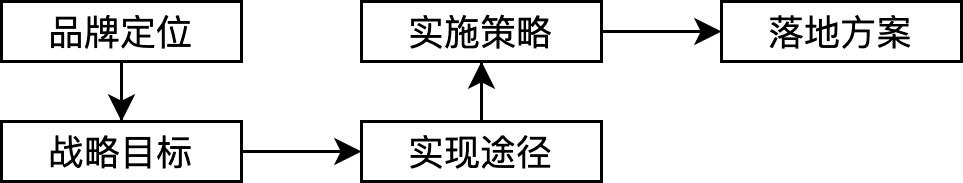
\includegraphics[width=\textwidth]{figures/1.png}
\caption{门头沟区综合考评品牌建设解决方案逻辑图}
\label{fig:fig1}
\end{figure}
\end{abstract}
\thispagestyle{empty}
\end{titlepage}

\newpage
\mbox{}
\thispagestyle{empty}
\newpage

\tableofcontents
\thispagestyle{empty}

\newpage
\mbox{}
\thispagestyle{empty}
\newpage

\newpage
\setcounter{page}{1}

\section{品牌定位}
根据普遍定义,政务品牌是指党政机关提供具有差异化的公共管理产品和服务,在社会公众或行政体系内部树立的地位、形象、威信,以及方针政策得到支持和贯彻的程度。

\subsection{政务品牌特点}
与商业品牌的定义相比,政务品牌具有两个共同的特点。一是业务的差异化和辨识度,用以区别于其他党政单位的同类化工作;二是文化承载功能,能够将零散的和碎片化的原则、理念、工作成效、影响力等因素高度聚合为价值文化。

与商业品牌的定义相比,政务品牌具有两个区别的特点。一是产品服务的公共性,这是由党政机关的公共部门属性决定的,政务品牌定位时将排除成本价格、市场竞争等影响因素;二是具有行政和管理功能,即在满足品牌受众相应需求的基础上,带有行政和管理的强制属性。

\subsection{品牌含义}
经研究,门头沟区综合考评政务品牌的含义应包括:深入结合门头沟区经济社会发展和党政治理体系等实际环境,由门头沟区综合考评办公室构建综合考评工作体系、提供综合考评工作方法、执行综合考评相关措施,在此过程中获得的有价值、有影响力、有长期效应的政绩成果,以及在门头沟区党政体系、门头沟区外综合考评业务领域和社会公众三个层面树立的形象、地位和威信(见图2)。
\begin{figure}[ht]
\centering
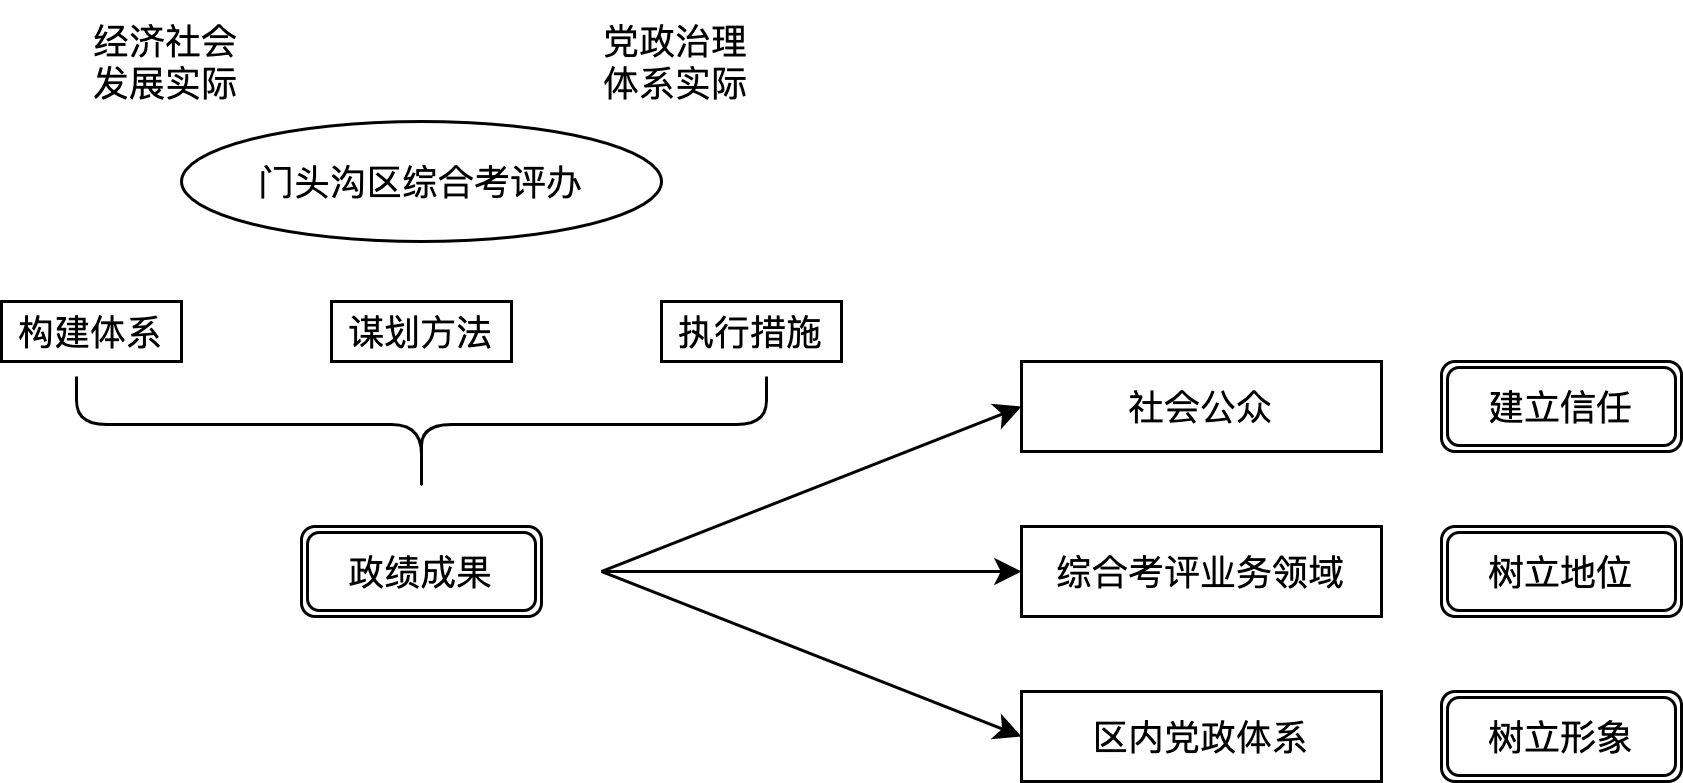
\includegraphics[width=\textwidth]{figures/2.png}
\caption{门头沟区综合考评品牌建设品牌含义解释图}
\label{fig:fig1}
\end{figure}

\section{品牌战略目标}
根据门头沟区综合考评工作实际以及相关业务的长期性质,建议按照构建品牌建设基础、树立品牌形象、扩大品牌影响力、维护品牌效应的合理顺序,分阶段设定品牌建设目标。品牌建设目标包括短期和长期两个阶段,能够为品牌建设保留良好的战略空间,保证战略实现的合理性和可操作性。

\subsection{短期目标(到2020年底)}
建议利用2020年全年,始终围绕“综合考评品牌建设”这个目标和方向,在一年内做好基础准备和框架构建,为“门头沟区综合考评”品牌建设提供必要的组织和机制保障(见图3)。
\begin{figure}[ht]
\centering
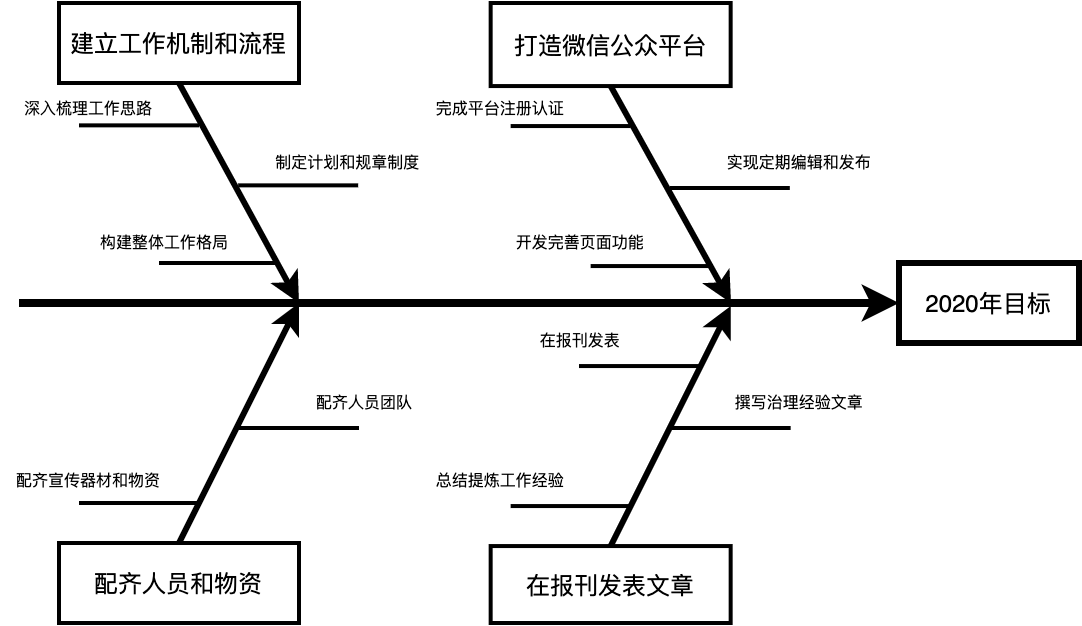
\includegraphics[width=\textwidth]{figures/3.png}
\caption{门头沟区综合考评品牌建设短期目标释义图}
\label{fig:fig1}
\end{figure}

一是深入梳理工作思路和方向,制定相应的宣传计划和规章制度,建立健全宣传工作机制和流程,创建综合考评宣传工作整体格局;

二是配备配齐器材物资和人员团队;

三是完成微信公众平台注册认证并实现内容的定期编辑与发布,开发并完善公众号页面功能;

四是在有影响力的相关报刊发表1篇关于门头沟区综合考评体系建设或工作成效的文章。

\subsection{长期目标(到2022年底)}
建议在三年内,通过党媒、期刊、微信公众号、视频发布渠道和线下会议活动等五个平台,在门头沟区党政机关内部、综合考评政务领域和社会公众三个层面,全方位打响具有门头沟区政务特色的综合考评政务品牌,并实现品牌质量的跟踪维护(见图4)。
\begin{figure}[ht]
\centering
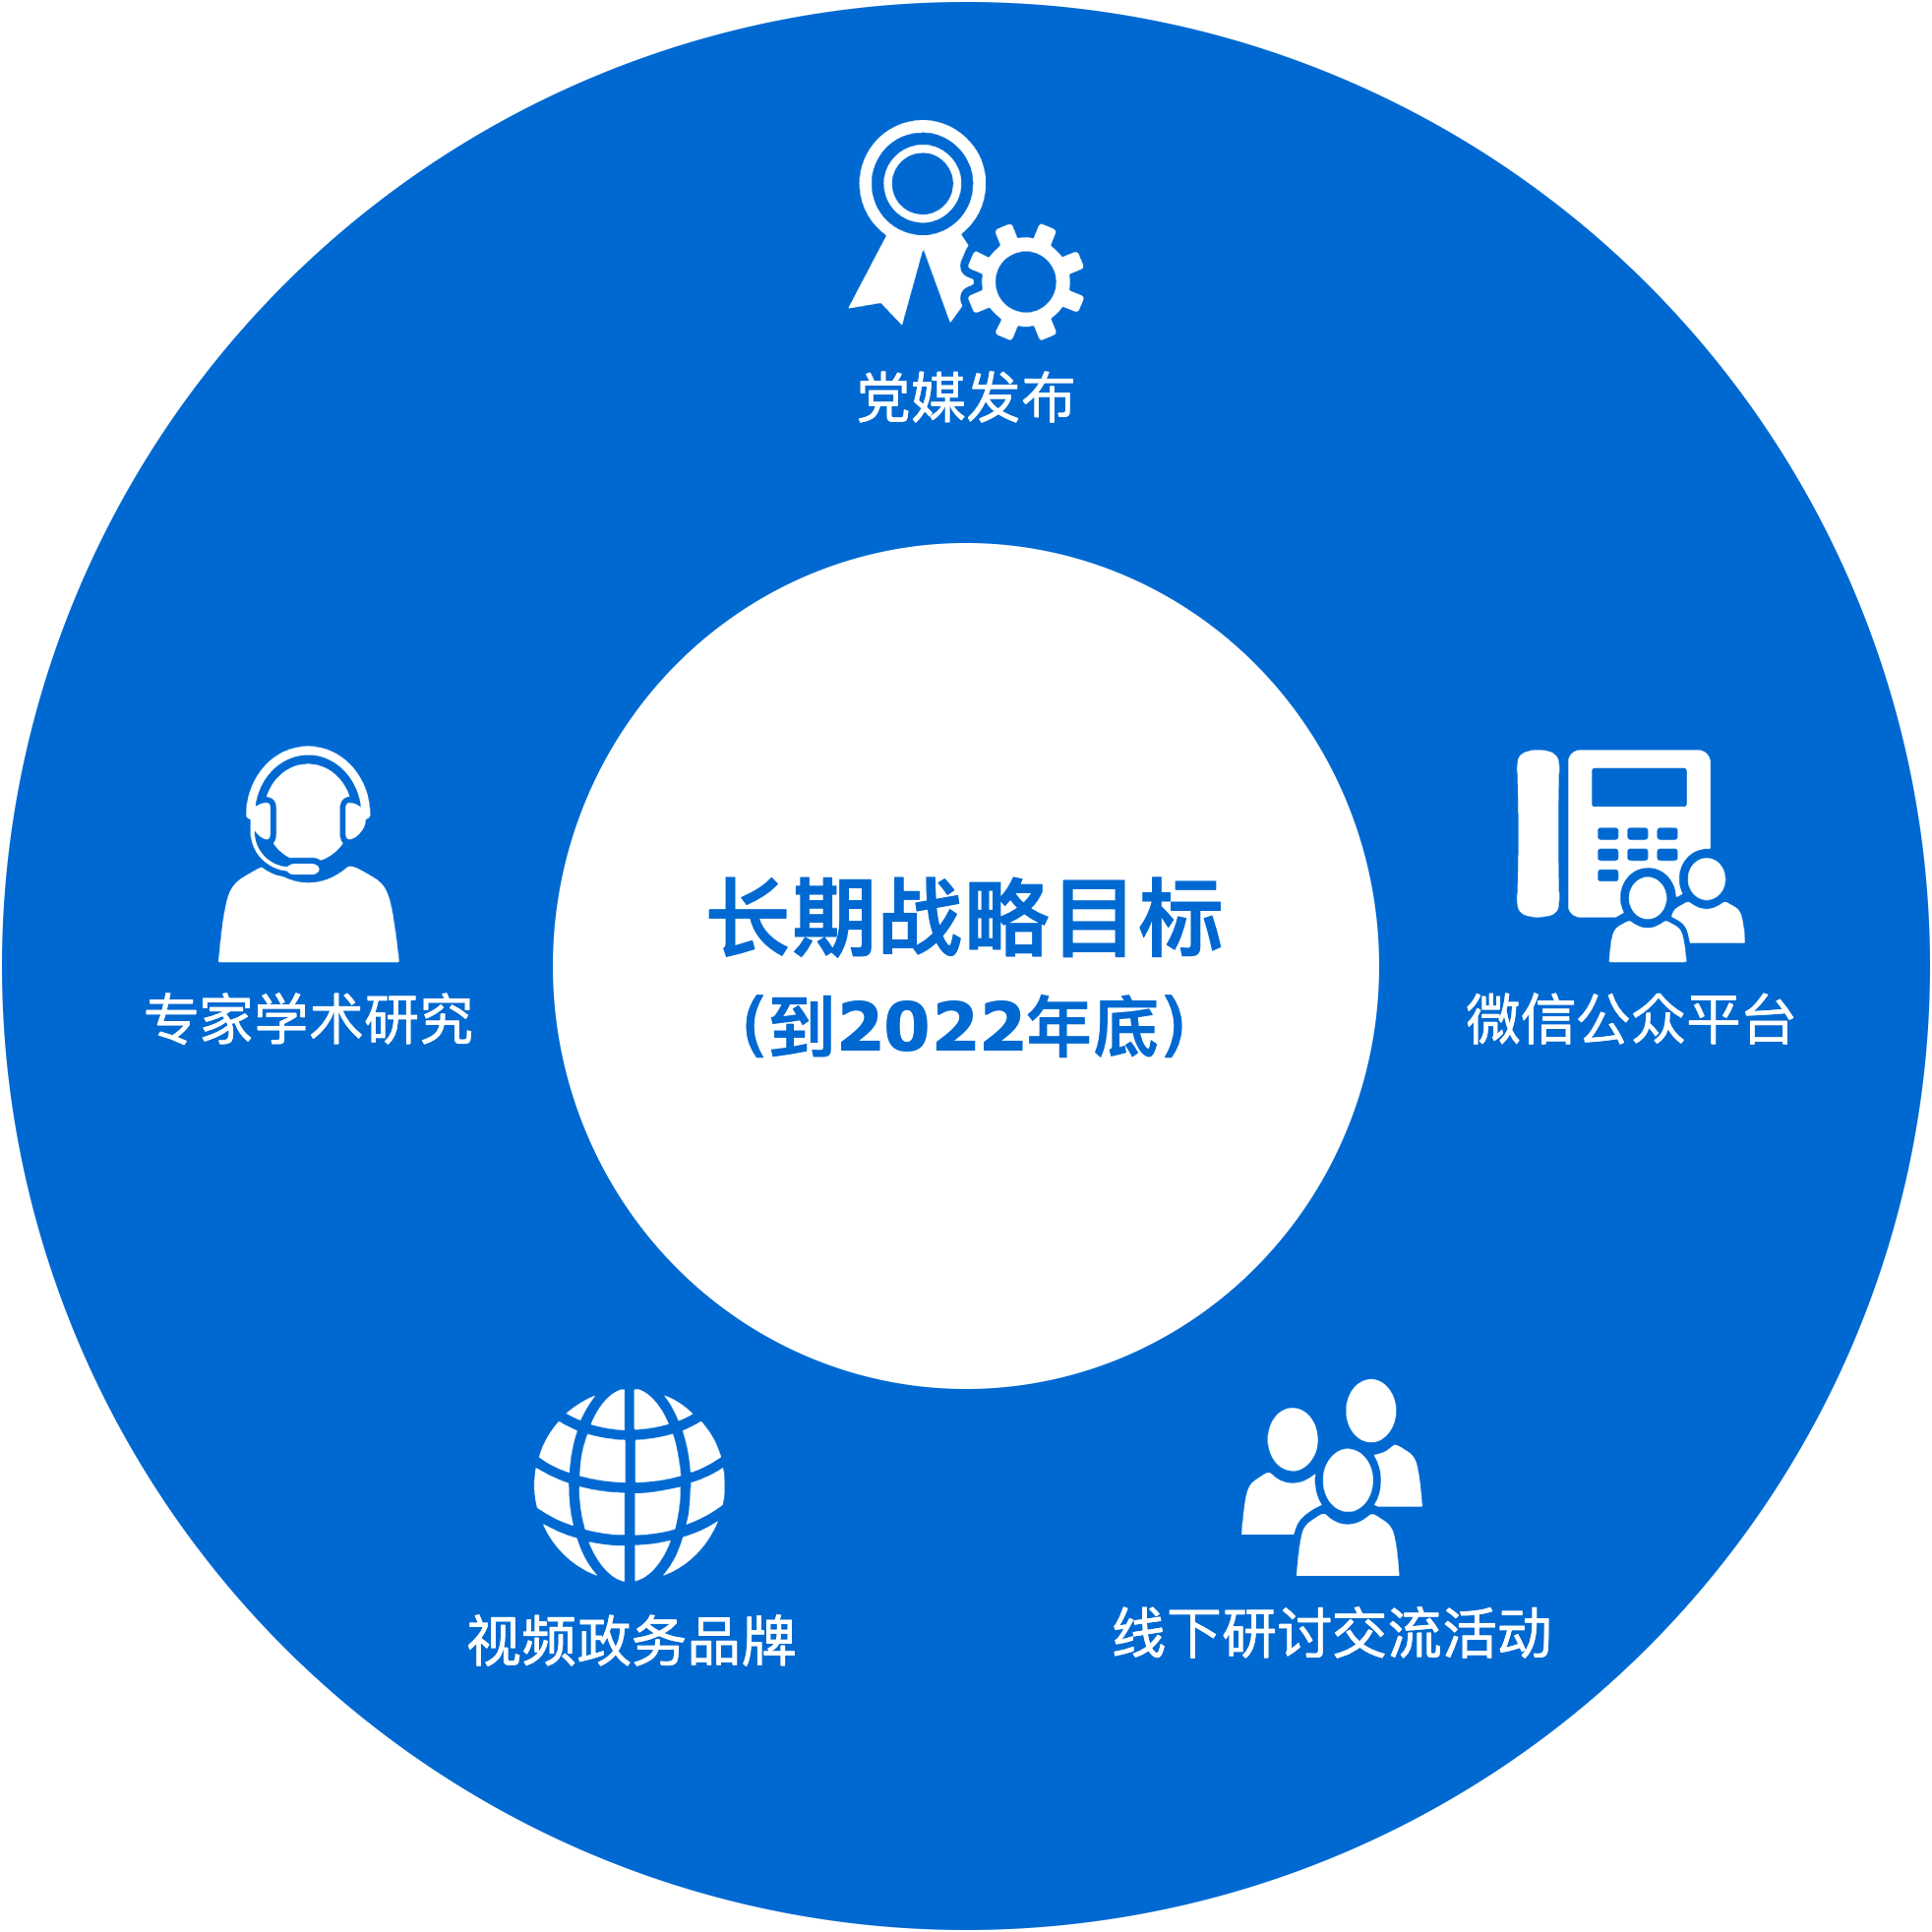
\includegraphics[width=\textwidth]{figures/4.png}
\caption{门头沟区综合考评品牌建设长期目标释义图}
\label{fig:fig1}
\end{figure}

一是围绕综合考评服务门头沟区发展全局、推动“绿水青山门头沟”和“红色门头沟”等战略实践的全过程,在中央和市级党媒成功发布报道,推广门头沟区综合考评工作的特色体系、经验做法和优良政绩;

二是通过专家学者的学术研究活动,高度总结并提炼综合考评工作在门头沟区治理体系和治理能力现代化过程中的重要作用,在有影响力的学术期刊成功发表相关理论成果;

三是将微信公众号打造成综合考评一体化平台,实现信息发布、成果展示、政民互动等功能,在党政机关内部和社会公众层面成功树立定位明确、主动作为、值得信任的政务影响力;

四是通过视频发布渠道,打造出具有一定社会影响力、形式多样、内容丰富的政务视频品牌;

五是在具有一定政绩成效和影响力的基础上,围绕“综合考评”相关主题,在市级或以上范围内成功组织并举办1次线下研讨交流活动。

\section{实现途径}
实现途径,是指为了完成品牌建设目标,基于基础业务和内部逻辑关系,从而规划的工作环节和业务流程。根据门头沟区综合考评工作实际,建议以考评业务为重要基础,以多样化宣传为重要手段,以分析反馈为提升渠道,构建三个环节的业务闭环——以业务基础作为宣传推广的内容核心和素材来源;在宣传推广过程中持续分析评判品牌建设效果,并反馈到业务运行环节;以分析反馈结果为重要参考,持续改进并完善业务工作、提出创新方法和模式(见图5)。
\begin{figure}[ht]
\centering
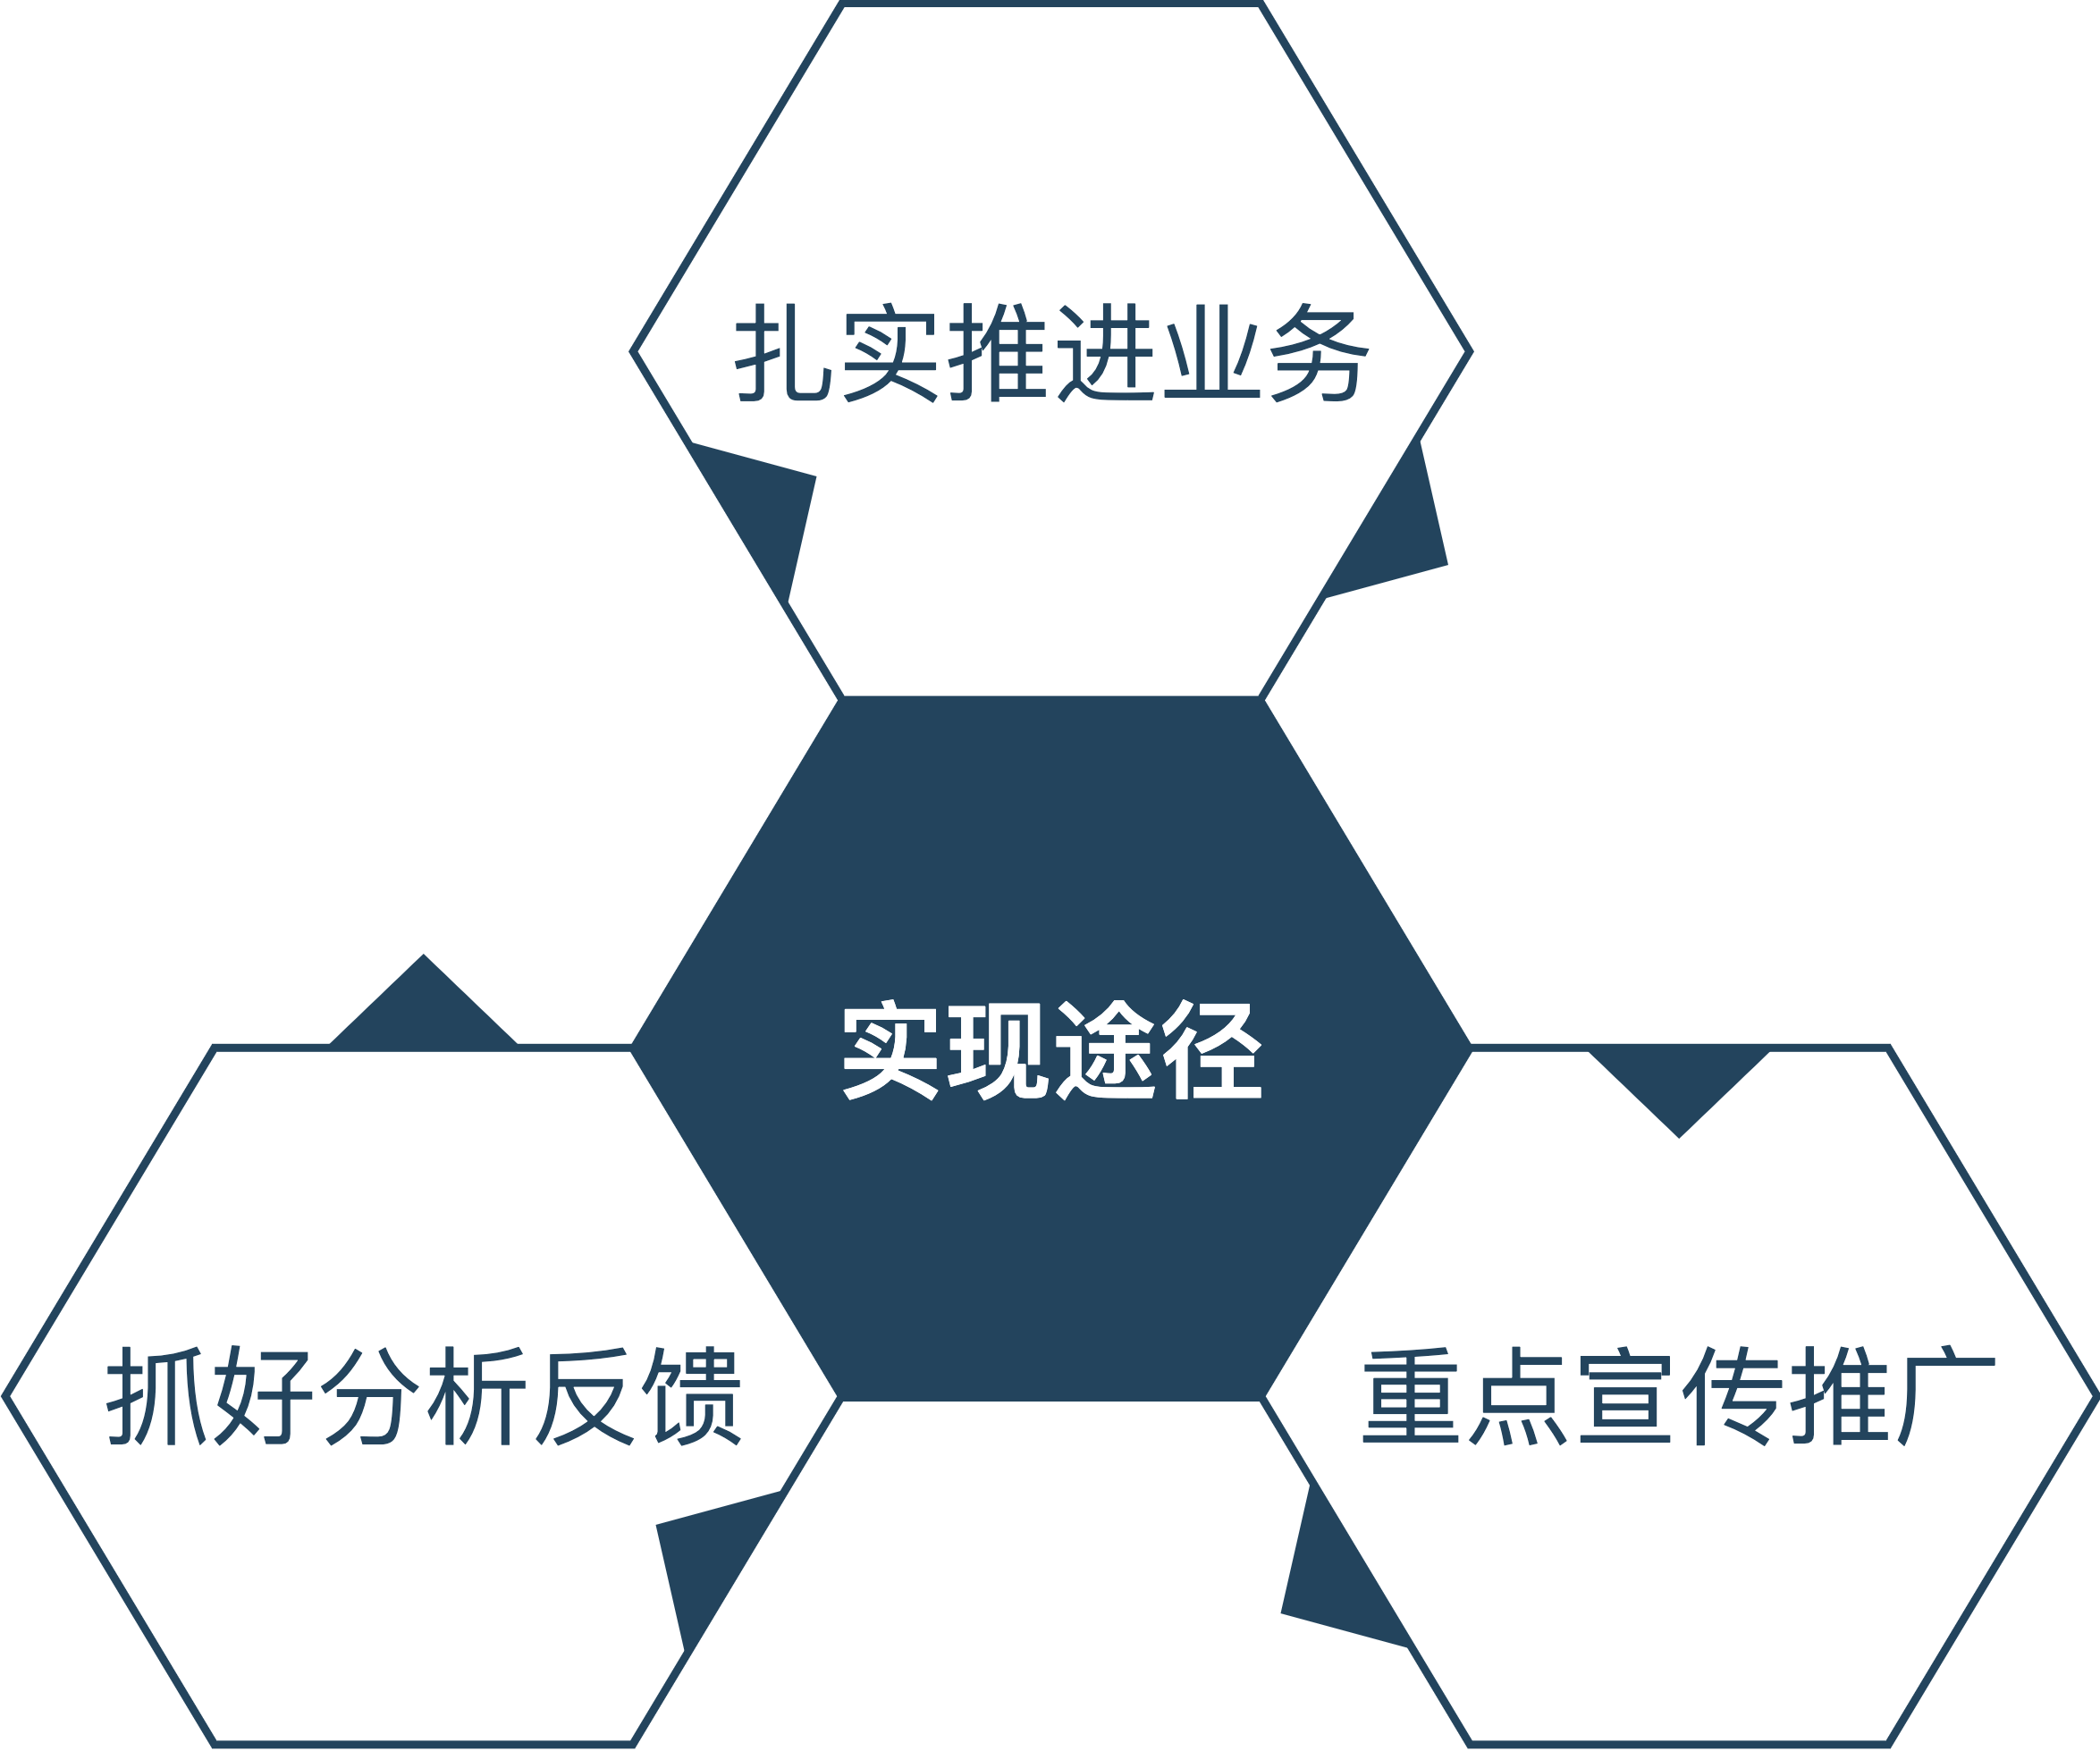
\includegraphics[width=\textwidth]{figures/5.png}
\caption{门头沟区综合考评品牌建设实现途径释义图}
\label{fig:fig1}
\end{figure}

\subsection{扎实推进业务,打好品牌基础}
业务工作是宣传推广的素材来源、文化理念的提炼原料和模式创新的根本基础。政务品牌建设建议稳步夯实业务基础,围绕《门头沟区2020年度综合考评工作要点》和各类纲领性文件,强化顶层设计、健全综合考评体制机制,强化过程管理、以考评推动工作高质量落实,紧抓关键环节、提升综合考评公正性和权威性,强化有效支撑、夯实综合考评工作基础。

同时,在综合考评业务运行过程中把握好宣传效果这个具体方向,围绕业务运行的主要内容,从各类工作主体收集业务素材,为下一步品牌推广工作奠定基础。

\subsection{运用宣传手段,开展品牌推广}
政务品牌主要以自发宣传为建设手段,运用各类宣传方法,将业务内容和文化理念向社会公众和特定范围推广。此处的宣传方法包括全面深入的政务公开、提纲挈领的经验总结、高度凝练的理论研究等等。

同时,在宣传推广的过程中,提供政务服务的主体能够通过相应方式收集并统计推广数据,为下一步分析反馈工作提供支撑。

\subsection{用好分析反馈,提升工作质量}
建议在收集并统计好推广数据的基础上,综合运用定量和定性的分析方法,从宣传本身和业务工作两方面展开分析,评估宣传效果和业务质量,总结提炼值得推广的工作经验、深入查摆存在不足的工作短板,并将分析结果及时反馈到品牌宣传和考评业务工作中,有效提升工作质量。

\section{实施策略}
在品牌建设具体实施的过程中,建议聚焦品牌短期和长期战略目标,围绕素材收集、内容加工、渠道发布等流程环节,重点抓好宣传推广工作(见表1)。
\begin{table}[ht]
\caption{门头沟区综合考评品牌建设实施策略一览表}
\label{tb:filter}
\centering
\begin{tabular}{c|c|l|l}
\hline
\multicolumn{2}{c|}{实施环节}    & \multicolumn{1}{c|}{短期内}                                                & \multicolumn{1}{c}{长期内}                                                                 \\ \hline
\multirow{3}{*}{素材收集} & 收集内容 & \begin{tabular}[c]{@{}l@{}}综合考评相关的政策文\\ 件、上级工作指示、本\\ 级工作动态\end{tabular} & \begin{tabular}[c]{@{}l@{}}延伸至街乡工作动态、其他省市区\\ 综合考评工作信息、与综合考评相\\ 关的学术成果和理论文献\end{tabular} \\ \cline{2-4} 
                      & 收集渠道 & \begin{tabular}[c]{@{}l@{}}政务信息公开渠道,以\\ 及宣传团队产出\end{tabular}            & \begin{tabular}[c]{@{}l@{}}拓展至区领导、门头沟区各街道和\\ 乡镇、综合考评相关的专家学者\end{tabular}                \\ \cline{2-4} 
                      & 收集方法 & 政策汇编、实时记录                                                               & \begin{tabular}[c]{@{}l@{}}政策汇编、实时记录、采访交流、\\ 文献研读、基层报送\end{tabular}                     \\ \hline
\multirow{2}{*}{内容加工} & 加工方式 & \begin{tabular}[c]{@{}l@{}}宣传团队选题策划和内\\ 部采写、编辑\end{tabular}             & \begin{tabular}[c]{@{}l@{}}邀请区领导和相应领域的专家、学\\ 者共同参与内容加工\end{tabular}                     \\ \cline{2-4} 
                      & 产出结果 & \begin{tabular}[c]{@{}l@{}}短篇通讯、政策解读、\\ 视频作品、数据报告\end{tabular}          & \begin{tabular}[c]{@{}l@{}}具有可操作性并且在理论和战略层\\ 面具有指导意义的内容\end{tabular}                    \\ \hline
\multirow{2}{*}{渠道发布} & 平台选择 & 党媒、微信公众平台                                                               & 拓展至抖音、b站、学术期刊                                                                           \\ \cline{2-4} 
                      & 发布强度 & \begin{tabular}[c]{@{}l@{}}传统党媒每季度稳定发\\ 布、公众号每周2-3篇\end{tabular}        & 根据当前品牌建设成效适时调整                                                                          \\ \hline
\end{tabular} 
\end{table}

\newpage
\subsection{素材收集环节}
素材收集环节是做好宣传推广的基础保障,能够为各类推广内容提供数据支撑、新闻来源和研究案例。根据门头沟区综合考评办公室当前实际,结合战略目标,从短期和长期两方面提出素材收集工作的具体实施策略。

1.短期(到2020年底)的素材收集工作建议着重考虑品牌建设起步阶段的实际情况,与宣传团队的人员数量和工作能力相匹配。

一是素材收集的内容,以综合考评相关的政策文件、上级工作指示、本级工作动态为主。

二是素材收集的渠道,主要包括北京市和门头沟区政务信息公开渠道,以及宣传团队收集或产出的文字、图片、数表和影像文件。

三是素材收集的方法,一方面定期整理并汇编相关政策文件,另一方面实时记录并拍摄工作内容。

2.长期(到2022年底)的素材收集工作建议着重考虑品牌效应,逐步拓宽收集内容和渠道的范围,综合运用各类方法提高收集效率。

一是素材收集的内容,在持续收集综合考评相关政策文件、上级工作指示、本级工作动态的基础上,关注范围可延伸至各街道和乡镇的综合考评工作动态、其他省市区综合考评工作信息、与综合考评相关的学术成果和理论文献。

二是素材收集的渠道,在用好各类政务信息公开渠道和宣传团队的基础上,收集渠道可拓展至区领导、门头沟区各街道和乡镇、综合考评相关的专家学者。

三是素材收集的方法,主要包括政策汇编、实时记录、采访交流、文献研读、基层报送等方式。

\subsection{内容加工环节}
内容加工是指对收集整理好的素材采取进一步归纳、分析、提炼,编辑并产出文章、音视频、图表等具有宣传价值的成果。根据门头沟区综合考评办公室当前实际,结合战略目标,从短期和长期两方面提出内容加工环节的具体实施策略。

1.短期(到2020年底)的内容加工建议着重发挥宣传团队的作用,稳步夯实工作人员的基本功,构建品牌建设的基本框架,有效避免相应的舆论风险。加工方式以宣传团队开展选题策划和内部采写、编辑为主,产出结果包括短篇通讯、政策解读、图片新闻、视频作品、成绩汇总、数据报告等内容。

2.长期(到2022年底)的内容加工建议着重体现专业化和理论化等特点,在宣传团队做好选题策划和内部采写、编辑的基础上,邀请区领导和相应领域的专家、学者共同参与内容加工,策划并产出具有可操作性并且在理论和战略层面具有指导意义的内容。

\subsection{渠道发布环节}
渠道发布是指将生产的内容通过特定方式以及相应渠道传播至社会公众的过程。根据门头沟区综合考评办公室当前实际,结合战略目标,从短期和长期两方面提出渠道发布环节的具体实施策略。

1.短期(到2020年底)的内容发布工作建议充分认识“品牌建立”起步阶段的重要特点,主要抓好传统党媒和微信公众平台两个渠道。一是坚守传统宣传阵地,着力在区级党报、党刊和卫视等渠道发布优质的宣传内容,发布强度建议保持每季度稳定发布;二是着力建设微信公众平台,将微信公众号打造成有初步影响力的权威发布渠道,同时为长期的品牌建设和维护打好基础,发布强度建议保持每周2至3篇宣传内容。

2.长期(到2022年底)的内容发布工作建议着重体现多元化特点,在持续做好传统党媒和微信公众号发布工作的同时,结合社会公众的多样化特点,综合运用抖音、b站、学术期刊等平台,以群众喜闻乐见的方式发布宣传内容,发布强度建议根据当前品牌建设成效适时调整。

此外,建议将举办线下研讨和交流会议等活动列入长期规划目标。在品牌建设初显成效且初具规模的阶段,在一定范围内(北京市各区、各地级市或其他直辖市区县)组织综合考评部门举办线下研讨和交流会议,能够作为高规格、高水平、高质量的发布渠道,公开展示门头沟区综合考评工作的政绩和成效,推广介绍相关文化理念和创新机制,体现门头沟区在推进治理体系和治理能力现代化过程中的探索,进一步扩大品牌影响。

\section{短期目标落地方案}
结合门头沟区综合考评工作实际,现将门头沟区2020年综合考评宣传工作策划如下。

\subsection{工作目标}
根据门头沟区综合考评办公室工作需求,元方智库组织人员研究后建议,开展2020年综合考评宣传工作应当始终围绕“综合考评品牌建设”这个目标和方向,做好基础准备和框架构建,为“门头沟区综合考评”品牌建设提供必要的组织和机制保障。
一是深入梳理工作思路和方向,出台相应的宣传计划和规章制度,建立健全宣传工作机制和流程,创建综合考评宣传工作整体格局;二是配备配齐器材物资和人员团队;三是完成微信公众平台注册认证并实现内容的定期编辑与发布,规划并开发公众号页面功能;四是在有影响力的相关报刊发表1篇关于门头沟区综合考评体系建设或工作成效的文章。
\subsection{宣传内容与范围}
根据门头沟区综合考评工作实际,2020年宣传内容和范围主要包括五个方面。
1.政策和解读。发布上级关于绩效管理和综合考评等文件的政策解读内容,包括党中央、国务院关于绩效管理和综合考评的相关文件,北京市关于绩效管理和综合考评的规定、指示和规划,以及各类专项文件和会议精神等内容。
2.访谈和文章。发布门头沟区综合考评工作的领导讲话,包括门头沟区主要领导关于综合考评工作的解读文章或访谈视频、专家学者关于综合考评和绩效管理的理论文章或访谈视频、考评对象负责人关于综合考评推动业务进展的体会文章或访谈视频等内容。
3.政务公开。一方面公示门头沟区综合考评相关文件,包括门头沟区2020年综合考评实施方案、各镇街关于综合考评的实施细则等内容;另一方面公示综合考评工作产生的各项成绩和结果,包括综合考评成绩、公众满意度评价情况、反馈整改进度和结果等内容。
4.工作动态。发布门头沟区综合考评工作实时动态,包括各级主要领导关于综合考评的工作新闻、各部门和镇街关于综合考评的工作内容、综合考评重要工作的落实情况以及综合考评宣传视频等内容。
5.政民互动情况。主要展示政民互动情况,包括社会公众来信解读、咨询答疑等内容,并利用宣传渠道开展社会评价调查等活动。
\subsection{实施流程}
本方案将围绕短期目标规划综合考评2020年宣传工作,主要目的在于打好基础、搭建框架、初见成效(见图6)。
\begin{figure}[ht]
\centering
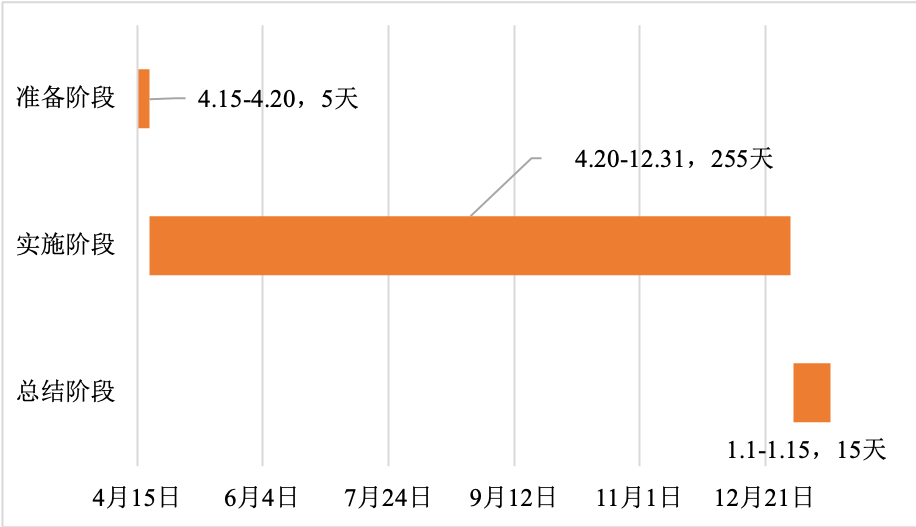
\includegraphics[width=\textwidth]{figures/6.png}
\caption{门头沟区综合考评品牌建设2020年实施进度图}
\label{fig:fig1}
\end{figure}

\newpage
\subsubsection{准备阶段}
准备阶段以规划设计、制定规章、组建团队为主,确保全年宣传工作有方向、有体系、有保障。准备阶段预计时间为2020年4月15日至4月20日。

1.规划宣传方向

一是邀请区领导和专家学者开展综合考评专题访谈,结合“绿水青山门头沟”和“红色门头沟党建”等发展理念,全面梳理并阐释门头沟区在短期和中长期的发展战略和实施路径,解读综合考评在各项战略目标实施过程中以及服务门头沟区发展全局的重要作用,深入挖掘门头沟区综合考评工作价值。

二是以区领导指示精神为依据,以专家学者的解读理论为参考,把握综合考评工作方针,进一步归纳综合考评宣传工作的整体方向。

三是以宣传方向为依据,全面深入地规划全年宣传工作各项细节,建议制定门头沟区2020年综合考评宣传工作计划,推动各方面工作稳步规范落实。

2.制定宣传条例

根据门头沟区政务公开、政务新媒体、政务宣传等方面的规章制度,以及门头沟区综合考评办公室相关要求,建议研究并制定门头沟区综合考评工作宣传条例,明确宣传原则、宣传内容、审批流程、舆论应急预案以及其他必要的工作标准,为宣传工作提供规范依据。

3.组建宣传团队

建议根据工作计划,设计并搭建综合考评宣传组织架构,包括领导小组、技术人员、编辑人员、审核人员、摄影摄像人员、美工设计人员、联络人员、服务保障人员和相应物资,确保涉及宣传的各方面基础工作职责明确、人员配位、物资齐全。

\subsubsection{实施阶段}

实施阶段以微信公众号注册、内容制作和发布为主,重点打造综合考评微信公众号,坚守并用好党媒宣传阵地,探索视频宣传等具有时代特点的新方法。实施阶段预计时间为2020年4月20日至12月31日。

4.建设微信公众号平台

建议充分认识微信公众号建设的重要意义,全力打造微信公众平台宣传阵地,借鉴“绩效杭州”等各类政务新媒体建设经验,清晰梳理公众号打造的规则流程、附带功能、发布内容类型等工作思路。

(1)工作步骤和方法

一是确定门头沟区综合考评品牌名称和图像标识,在微信公众平台注册并完成主体认证;二是根据实际需求和工作目标,设计并开发公众号附带功能,完善公众号建设框架;三是开展公众号品牌推广,实现读者引流;四是按照相关规定和文件,根据工作实际稳定发布综合考评信息和内容;五是根据群众反馈的信息,实时开展用户分析,持续改进宣传工作。

(2)明确发布内容

通过微信公众平台,定期组织内部编辑、门沟头区机关单位和乡镇街道,发布文章、图片、音频、视频等各类信息。发布的具体内容和时间由门头沟区综合考评办公室确定。

(3)开发平台功能

平台开发是指利用微信公众平台的特点,设计公众号的展示页面,开发实用的附属功能。公众号页面建议开发“考评讲堂”“考评动态”“考评公示”“互动平台”等栏目,分别对应相关发布内容。

具体的功能开发以门头沟区综合考评办公室需求为标准,建议以打造“综合考评工作一体化平台”为目标,开发会员注册、事项投票、问卷发布、留言互动等功能,为中长期品牌建设目标打好基础。

(4)实现平台引流

完成公众号注册和认证后,需要通过相关方法进行用户引流,完成一定数量的用户关注。建议通过门头沟区现有的政务新媒体进行推广,通过发布重要文件和优质内容实现一定范围的自主传播,或在政府机关内部动员相关人员进行转发、推广,在一定时间内实现预期数量的用户关注。

(5)分析互动信息

微信公众号自带的后台留言功能在一定程度上能够实现平台和用户之间的互动。建议定期汇总宣传受众的反馈信息并开展内容分析,查摆综合考评工作存在的问题,研究改进方法。另一方面,建议根据反馈信息,提前研判综合考评工作面临的社会环境和政务环境发展趋势,主动寻求革新和改变。

5.坚守党媒阵地

要重视党报、党刊、地方卫视等党媒作为传统宣传阵地的重要作用。建议结合综合考评工作特点,根据门头沟区区领导指示和综合考评办公室工作实际,于重要的时间节点,在区级媒体发布合适的宣传内容,向社会公布工作动态,总结并展示工作亮点。一是发布当年综合考评实施方案;二是发布当年综合考评成绩;三是发布当年综合考评社会评价情况;四是发布门头沟区领导干部关于综合考评工作的指示或思路;五是发布专家学者对于门头沟区综合考评工作特色的专题解读;六是发布门头沟区开展综合考评工作的创新思路、工作亮点、成熟模式、机制体系等内容,纵向挖掘综合考评工作价值。

传统媒体发布平台选择和发布内容根据门头沟区党媒情况实际,由门头沟区综合考评办公室确定。

6.探索宣传新方法

在做好传统媒体和微信公众平台的同时,建议充分结合门头沟区综合考评工作实际,探索短视频、宣传片等创新方法,在抖音等新媒体平台打造综合考评宣传矩阵。

\subsubsection{分析总结阶段}
分析总结阶段是指对综合考评全年宣传工作进行分析,为更好地开展下阶段宣传工作、完成综合考评宣传中长期目标提供相关对策建议和保障。分析总结阶段预计时间为2021年1月1日至1月15日。

7.分析总结并研究对策

建议围绕宣传工作做好全年总结和研究分析工作。一是查找梳理工作存在的不足,包括宣传工作过程中存在的问题,以及通过宣传反馈发现的综合考评工作存在缺陷;二是总结提炼优秀经验做法,在深入总结的基础上,将具有实用价值和推广价值的宣传措施和方法提炼成型;三是研究制定提升改进方法,纠正、改善有缺陷的工作流程和方法,提出进一步创新和提升的意见。

8.梳理群众意见

针对社会公众在宣传互动中提出的意见建议,建议及时梳理汇总并加以研判。情况属实、性质重要的意见,经领导审批后反馈至相关工作部门和单位,研究后纳入综合考评体系。

9.开展战略研判

在完成全年宣传工作既定目标的基础上,建议聚焦品牌建设,从业务本身和宣传工作两方面分析并评估综合考评品牌建设成效,判断宣传工作战略进展情况,研究并调整2021年和接下来一段时间的工作计划和战略目标。

\subsection{工作原则}
\subsubsection{注重纪律性}
宣传是党政工作的重要部分,建议在宣传工作过程中明确并时刻遵守宣传纪律,明确规定审批流程、统一宣传口径、严格审核标准,确保宣传工作不出差错,避免过度宣传、虚假宣传、泄密事件和风险事件。

\subsubsection{注重时效性}
建议重视宣传发布的时效性,时刻保持宣传工作的组织效率和工作人员的尽责态度,及时将综合考评相关内容整理发布,确保社会公众和党政机关工作人员第一时间接收门头沟区综合考评的政策文件和工作动态。

\subsubsection{注重可读性}
通过打造宣传矩阵的方式开展宣传工作,建议重视宣传内容的可读性,根据发布渠道的内容要求和受众人群特点适当调整宣传风格,避免过度使用“空话”“大话”“套话”,通过浅显易懂的文字、图表、音视频等方式向社会群众发布有关内容。

\end{document}
